\documentclass[11pt,fleqn]{article}
\usepackage[cm]{fullpage}
%%AVC PACKAGES
\usepackage{avcgreek}
\usepackage{avcfonts}
\usepackage{avcmath}
\usepackage[numberby=section]{avcthm} % 
\usepackage{qcmacros}
\usepackage{goldstone}
%%MACROS FOR THIS DOCUMENT
\numberwithin{equation}{section}
\usepackage{titlesec}
\titleformat{\section}{\Large\bfseries\mathversion{bold}}{\thesection.}{5pt}{}
% remove header from TOC
\makeatletter
\renewcommand\tableofcontents{%
  \@starttoc{toc}%
}
\makeatother


%%%DOCUMENT%%%
\begin{document}

\section{Diagram notation (draft)}

\begin{ntt}
\thmtitle{Particle-hole operators in diagram notation}
In diagram notation, particle-hole operators are written as oriented lines extending from a vertex.
Particle annihilation operators enter the vertex from below, particle creation operators leave the vertex extending upward, and single-excitation operators have both creation and annihilation lines.
Contractions of are represented by joining particle-hole lines with compatible position and orientation.
\begin{align*}
&&
\diagram{
  \node[dot=white,label=above:$p$] (p) at (0,0) {};
  \draw[-<-] (p) to ++(0,-0.5);
}
\equiv
  a_p
&&
\diagram{
  \node[dot=white,label=below:$p$] (p) at (0,0) {};
  \draw[->-] (p) to ++(0,+0.5);
}
\equiv
  a_p^\dagger
&&
\diagram{
  \node[dot=white] (a) at (0,0) {};
  \draw[->-] (a) to ++(0,+0.5) node[above] {$p$};
  \draw[-<-] (a) to ++(0,-0.5) node[below] {$q$};
}
\equiv
  a_p\dg a_q
&&
\diagram{
  \node[dot=white,label=above:$p$] (p) at (0,+0.5) {};
  \node[dot=white,label=below:$q$] (q) at (0,-0.5) {};
  \draw[->-] (q) to (p);
}
\equiv
  \ctr{}{a}{_p}{a} a_p a_q\dg
=
  \d_{pq}
\end{align*}
Note that the vanishing contractions are not expressible in diagram notation.
This has the advantage of simplifying the evaluation of Wick expansions without any loss of generality.
\end{ntt}

\begin{rmk}
\thmtitle{Spin-orbital labels in diagram notation}
When using generic placeholder indices, the spin-orbital labels are dispensed with wherever possible.
The removal of placeholder indices supports the primary objective of diagram notation:
stripping an expression of all extraneous details to reveal its essential information content.
\begin{align*}
&&
\diagram{
  \node[dot=white] (p) at (0,0) {};
  \draw[-<-] (p) to ++(0,-0.5);
}
\mapsto
  a_p
&&
\diagram{
  \node[dot=white] (p) at (0,0) {};
  \draw[->-] (p) to ++(0,+0.5);
}
\mapsto
  a_p^\dagger
&&
\diagram{
  \node[dot=white] (a) at (0,0) {};
  \draw[->-] (a) to ++(0,+0.5);
  \draw[-<-] (a) to ++(0,-0.5);
}
\mapsto
  a_p\dg a_q
&&
\diagram{
  \node[dot=white] (p) at (0,+0.5) {};
  \node[dot=white] (q) at (0,-0.5) {};
  \draw[->-] (q) to (p);
}
\mapsto
  \ctr{}{a}{_p}{a} a_p a_q\dg
\end{align*}
\end{rmk}

\begin{ntt}
\thmtitle{Quasiparticle-quasihole operators in diagram notation}
Diagram notation with respect to $\F$ is expressed in the quasiparticle operator basis, which is indicated by the use of closed- rather than open-circle vertices.
For particles, annihilation operators enter the vertex from below while creation operators leave the vertex extending upward.
For holes, annihilation operators leave the vertex extending downward while creation operators enter from above.
\begin{align*}
&&
\diagram{
  \node[dot] (a) at (0,0) {};
  \draw[-<-] (a) to ++(0,-0.5);
}
\mapsto
  b_a
&&
\diagram{
  \node[dot] (a) at (0,0) {};
  \draw[->-] (a) to ++(0,+0.5);
}
\mapsto
  b_a^\dagger
&&
\diagram{
  \node[dot] (i) at (0,0) {};
  \draw[->-] (i) to ++(0,-0.5);
}
\mapsto
  b_i
&&
\diagram{
  \node[dot] (i) at (0,0) {};
  \draw[-<-] (i) to ++(0,+0.5);
}
\mapsto
  b_i^\dagger
\end{align*}
That is, the hole operator diagrams are rotated by $180^\circ$.
In this basis, there are two possible contractions
\begin{align*}
&&
\diagram{
  \node[dot] (a) at (0,+0.5) {};
  \node[dot] (b) at (0,-0.5) {};
  \draw[->-] (b) to (a);
}
\mapsto
  \ctr{}{b}{_a}{b}  b_ab_b\dg
&&
\diagram{
  \node[dot] (i) at (0,+0.5) {};
  \node[dot] (j) at (0,-0.5) {};
  \draw[-<-] (j) to (i);
}
\mapsto
  \ctr{}{b}{_i}{b}  b_ib_j\dg
\end{align*}
and the single-excitation operator $a_p\dg a_q$ splits into four distinct parts.
\begin{align*}
&&
\diagram{
  \node[dot] (ab) at (0,0) {};
  \draw[->-] (ab) to ++(0,+0.5);
  \draw[-<-] (ab) to ++(0,-0.5);
}
\mapsto
  b_a\dg b_b
=
  a_a\dg a_b
&&
\diagram{
  \node[dot] (ai) at (0,0) {};
  \draw[->-] (ai) to ++(-0.25,+0.5);
  \draw[-<-] (ai) to ++(+0.25,+0.5);
}
\mapsto
  b_a\dg b_i\dg
=
  a_a\dg a_i
&&
\diagram{
  \node[dot] (ia) at (0,0) {};
  \draw[->-] (ia) to ++(-0.25,-0.5);
  \draw[-<-] (ia) to ++(+0.25,-0.5);
}
\mapsto
  b_ib_a
=
  a_i\dg a_a
&&
\diagram{
  \node[dot] (ij) at (0,0) {};
  \draw[-<-] (ij) to ++(0,+0.5);
  \draw[->-] (ij) to ++(0,-0.5);
}
\mapsto
  b_ib_j\dg 
=
  a_i\dg a_j
\end{align*}
\end{ntt}

\begin{dfn}
\thmtitle{Bubble contractions}
A \textit{bubble contraction} is an internal contraction of a single-excitation operator.
\begin{align*}
&&
\diagram{
  \node[dot] (pq) at (0,0) {};
  \draw[->-] (pq) arc (0:360:+0.3) {};
}
\mapsto
  \ctr{}{b}{_i}{b}  b_ib_j\dg
\end{align*}
By convention bubble contractions are defined to represent only hole contractions, since excitation operators have no internal particle contractions.
\end{dfn}


\begin{ex}
The \vac-normal Wick expansion of $a_pa_q\dg$ can be expressed diagram notation as follows.
\begin{align*}
&&
    a_pa_q\dg
  =
  -
    a_q\dg a_p
  +
    \ctr{}{a}{_p}{a} a_pa_q\dg
\hspace{20pt}\leftrightarrow\hspace{20pt}
  \diagram{
    \node[dot=white] (p) at (0,+0.55) {};
    \node[dot=white] (q) at (0,-0.55) {};
    \draw[-<-] (p) to ++(0,-0.5);
    \draw[->-] (q) to ++(0,+0.5);
  }
  =
  -
  \diagram{
    \node[dot=white] (pq) at (0,0) {};
    \draw[->-] (pq) to ++(0,+0.5);
    \draw[-<-] (pq) to ++(0,-0.5);
  }
  +
  \diagram{
    \node[dot=white] (p) at (0,+0.5) {};
    \node[dot=white] (q) at (0,-0.5) {};
    \draw[->-] (q) to (p);
  }
\end{align*}
Note that the operators in a diagram are ordered from top-to-bottom rather than left-to-right [fig~\ref{fig:diagram-example}(a)].
\end{ex}

\begin{ntt}
\thmtitle{Diagram notation for $\vac$- and $\F$-normal-ordered excitation operators}
\vac-normal-ordered excitation operators are expressed in diagram notation as single-excitation operators connected by a line.
$\F$-normal-ordered excitation operators are distinguished from $\vac$-normal-ordered ones by using double-circle vertices.
\begin{align*}
&&
\diagram{
  \node[dot=white] (a1) at (0,0) {};
  \node[dot=white] (a2) at (1,0) {};
  \node (dots) at (1.75,0) {$\cdots$};
  \node[dot=white] (an) at (2.5,0) {};
  \draw (a1)--(a2)--(dots)--(an);
  \draw[->-] (a1) to ++(0,+0.5);
  \draw[->-] (a2) to ++(0,+0.5);
  \draw[->-] (an) to ++(0,+0.5);
  \draw[-<-] (a1) to ++(0,-0.5) coordinate[below left=0.1cm and 0.1cm] (startbrace);
  \draw[-<-] (a2) to ++(0,-0.5);
  \draw[-<-] (an) to ++(0,-0.5) coordinate[below right=0.1cm and 0.1cm] (endbrace);
  \draw[decorate,decoration={brace,mirror}] (startbrace) to node[midway,below=0.1cm] () {\scriptsize{$m$ times}} (endbrace);
}
\mapsto
  \no{a^{p_1}_{q_1}a^{p_2}_{q_2}\cd a^{p_m}_{q_m}}
=
  a^{p_1\cd p_m}_{q_1\cd q_m}
&&
\diagram{
  \node[ddot=white] (a1) at (0,0) {};
  \node[ddot=white] (a2) at (1,0) {};
  \node (dots) at (1.75,0) {$\cdots$};
  \node[ddot=white] (an) at (2.5,0) {};
  \draw (a1)--(a2)--(dots)--(an);
  \draw[->-] (a1) to ++(0,+0.5);
  \draw[->-] (a2) to ++(0,+0.5);
  \draw[->-] (an) to ++(0,+0.5);
  \draw[-<-] (a1) to ++(0,-0.5) coordinate[below left=0.1cm and 0.1cm] (startbrace);
  \draw[-<-] (a2) to ++(0,-0.5);
  \draw[-<-] (an) to ++(0,-0.5) coordinate[below right=0.1cm and 0.1cm] (endbrace);
  \draw[decorate,decoration={brace,mirror}] (startbrace) to node[midway,below=0.1cm] () {\scriptsize{$m$ times}} (endbrace);
}
\mapsto
  \gno{a^{p_1}_{q_1}a^{p_2}_{q_2}\cd a^{p_m}_{q_m}}
=
  \tl{a}^{p_1\cd p_m}_{q_1\cd q_m}
\end{align*}
Here too internal contractions of the diagram are defined to represent hole contractions.
\end{ntt}


\begin{ntt}
\thmtitle{Diagram notation for normal-ordered products of excitation operators}
A pair of excitation operators connected by one or more cross-contractions is implicitly normal-ordered together.
\begin{align*}
\diagram{
% first excitation operator
  \node[dot=white] (a1) at (0,0.5) {};
  \node[dot=white] (a2) at (1,0.5) {};
  \node (dots) at (1.75,0.5) {$\cdots$};
  \node[dot=white] (an) at (2.5,0.5) {};
  \draw (a1)--(a2)--(dots)--(an);
  \draw[->-] (a1) to ++(0,+0.5) coordinate[above left=0.1cm and 0.1cm] (startbrace);
  \draw[->-] (a2) to ++(0,+0.5);
  \draw[->-] (an) to ++(0,+0.5) coordinate[above right=0.1cm and 0.1cm] (endbrace);
  \draw[-<-] (a1) to ++(0,-0.5);
  \draw[-<-] (a2) to ++(0,-0.5);
  \draw[decorate,decoration={brace}] (startbrace) to node[midway,above=0.1cm] () {\scriptsize{$m$ times}} (endbrace);
% second excitation operator
  \node[dot=white] (b1) at (2.5,-0.5) {};
  \node[dot=white] (b2) at (3.5,-0.5) {};
  \node (dots2) at (4.25,-0.5) {$\cdots$};
  \node[dot=white] (bn) at (5.0,-0.5) {};
  \draw (b1)--(b2)--(dots2)--(bn);
  \draw[->-] (b2) to ++(0,+0.5);
  \draw[->-] (bn) to ++(0,+0.5);
  \draw[-<-] (b1) to ++(0,-0.5) coordinate[below left=0.1cm and 0.1cm] (startbrace2);
  \draw[-<-] (b2) to ++(0,-0.5);
  \draw[-<-] (bn) to ++(0,-0.5) coordinate[below right=0.1cm and 0.1cm] (endbrace2);
  \draw[decorate,decoration={brace,mirror}] (startbrace2) to node[midway,below=0.1cm] () {\scriptsize{$n$ times}} (endbrace2);
% connecting line
  \draw[->-] (b1)--(an);
}
\mapsto
  \no{a^{p_1\cd p_m}_{q_1\cd q_m^\hole}a^{r_1^\hole\cd r_n}_{s_1\cd s_n}}
&&
\hspace{15pt}
\diagram{
% first excitation operator
  \node[ddot=white] (a1) at (0,0.5) {};
  \node[ddot=white] (a2) at (1,0.5) {};
  \node (dots) at (1.75,0.5) {$\cdots$};
  \node[ddot=white] (an) at (2.5,0.5) {};
  \draw (a1)--(a2)--(dots)--(an);
  \draw[->-] (a1) to ++(0,+0.5) coordinate[above left=0.1cm and 0.1cm] (startbrace);
  \draw[->-] (a2) to ++(0,+0.5);
  \draw[->-] (an) to ++(0,+0.5) coordinate[above right=0.1cm and 0.1cm] (endbrace);
  \draw[-<-] (a1) to ++(0,-0.5);
  \draw[-<-] (a2) to ++(0,-0.5);
  \draw[decorate,decoration={brace}] (startbrace) to node[midway,above=0.1cm] () {\scriptsize{$m$ times}} (endbrace);
% second excitation operator
  \node[ddot=white] (b1) at (2.5,-0.5) {};
  \node[ddot=white] (b2) at (3.5,-0.5) {};
  \node (dots2) at (4.25,-0.5) {$\cdots$};
  \node[ddot=white] (bn) at (5.0,-0.5) {};
  \draw (b1)--(b2)--(dots2)--(bn);
  \draw[->-] (b2) to ++(0,+0.5);
  \draw[->-] (bn) to ++(0,+0.5);
  \draw[-<-] (b1) to ++(0,-0.5) coordinate[below left=0.1cm and 0.1cm] (startbrace2);
  \draw[-<-] (b2) to ++(0,-0.5);
  \draw[-<-] (bn) to ++(0,-0.5) coordinate[below right=0.1cm and 0.1cm] (endbrace2);
  \draw[decorate,decoration={brace,mirror}] (startbrace2) to node[midway,below=0.1cm] () {\scriptsize{$n$ times}} (endbrace2);
% connecting line
  \draw[->-] (b1)--(an);
}
\mapsto
  \gno{a^{p_1\cd p_m}_{q_1\cd q_m^\hole}a^{r_1^\hole\cd r_n}_{s_1\cd s_n}}
\end{align*}
When excitation operators without cross-contractions are normal ordered together, this is indicated by connecting them with a horizontal dotted line.
\begin{align*}
\diagram{
% first excitation operator
  \node[dot=white] (a1) at (0,0) {};
  \node[dot=white] (a2) at (1,0) {};
  \node (dots) at (1.75,0) {$\cdots$};
  \node[dot=white] (an) at (2.5,0) {};
  \draw (a1)--(a2)--(dots)--(an);
  \draw[->-] (a1) to ++(0,+0.5);
  \draw[->-] (a2) to ++(0,+0.5);
  \draw[->-] (an) to ++(0,+0.5);
  \draw[-<-] (a1) to ++(0,-0.5) coordinate[below left=0.1cm and 0.1cm] (startbrace);
  \draw[-<-] (a2) to ++(0,-0.5);
  \draw[-<-] (an) to ++(0,-0.5) coordinate[below right=0.1cm and 0.1cm] (endbrace);
  \draw[decorate,decoration={brace,mirror}] (startbrace) to node[midway,below=0.1cm] () {\scriptsize{$m$ times}} (endbrace);
% second excitation operator
  \node[dot=white] (b1) at (3.5,0) {};
  \node[dot=white] (b2) at (4.5,0) {};
  \node (dots2) at (5.25,0) {$\cdots$};
  \node[dot=white] (bn) at (6.0,0) {};
  \draw (b1)--(b2)--(dots2)--(bn);
  \draw[->-] (b1) to ++(0,+0.5);
  \draw[->-] (b2) to ++(0,+0.5);
  \draw[->-] (bn) to ++(0,+0.5);
  \draw[-<-] (b1) to ++(0,-0.5) coordinate[below left=0.1cm and 0.1cm] (startbrace2);
  \draw[-<-] (b2) to ++(0,-0.5);
  \draw[-<-] (bn) to ++(0,-0.5) coordinate[below right=0.1cm and 0.1cm] (endbrace2);
  \draw[decorate,decoration={brace,mirror}] (startbrace2) to node[midway,below=0.1cm] () {\scriptsize{$n$ times}} (endbrace2);
% connecting line
  \draw[densely dotted] (an)--(b1);
}
\mapsto
  \no{a^{p_1\cd p_m}_{q_1\cd q_m}a^{r_1\cd r_n}_{s_1\cd s_n}}
&&
\hspace{15pt}
\diagram{
% first excitation operator
  \node[ddot=white] (a1) at (0,0) {};
  \node[ddot=white] (a2) at (1,0) {};
  \node (dots) at (1.75,0) {$\cdots$};
  \node[ddot=white] (an) at (2.5,0) {};
  \draw (a1)--(a2)--(dots)--(an);
  \draw[->-] (a1) to ++(0,+0.5);
  \draw[->-] (a2) to ++(0,+0.5);
  \draw[->-] (an) to ++(0,+0.5);
  \draw[-<-] (a1) to ++(0,-0.5) coordinate[below left=0.1cm and 0.1cm] (startbrace);
  \draw[-<-] (a2) to ++(0,-0.5);
  \draw[-<-] (an) to ++(0,-0.5) coordinate[below right=0.1cm and 0.1cm] (endbrace);
  \draw[decorate,decoration={brace,mirror}] (startbrace) to node[midway,below=0.1cm] () {\scriptsize{$m$ times}} (endbrace);
% second excitation operator
  \node[ddot=white] (b1) at (3.5,0) {};
  \node[ddot=white] (b2) at (4.5,0) {};
  \node (dots2) at (5.25,0) {$\cdots$};
  \node[ddot=white] (bn) at (6.0,0) {};
  \draw (b1)--(b2)--(dots2)--(bn);
  \draw[->-] (b1) to ++(0,+0.5);
  \draw[->-] (b2) to ++(0,+0.5);
  \draw[->-] (bn) to ++(0,+0.5);
  \draw[-<-] (b1) to ++(0,-0.5) coordinate[below left=0.1cm and 0.1cm] (startbrace2);
  \draw[-<-] (b2) to ++(0,-0.5);
  \draw[-<-] (bn) to ++(0,-0.5) coordinate[below right=0.1cm and 0.1cm] (endbrace2);
  \draw[decorate,decoration={brace,mirror}] (startbrace2) to node[midway,below=0.1cm] () {\scriptsize{$n$ times}} (endbrace2);
% connecting line
  \draw[densely dotted] (an)--(b1);
}
\mapsto
  \gno{a^{p_1\cd p_m}_{q_1\cd q_m}a^{r_1\cd r_n}_{s_1\cd s_n}}
\end{align*}
For excitation operators these can obviously be replaced by solid lines, but this distinction will become important when the excitation operators are replaced with $m$-electron operators.
\end{ntt}

\begin{dfn}\label{dfn:m-electorn-operators-antisymmetric-interaction-tensors}
\thmtitle{$m$-electron operators, antisymmetric interaction tensors}
The fundamental components of a diagram (\Cref{dfn:diagram}) are \textit{$m$-electron operators} with \textit{antisymmetric interaction tensors}.
That is, operators of the form
\begin{align*}
&&
  V
=
  \pr{\tfr{1}{m!}}^2
  \sum_{\text{Einstein}}
  \ol{v}_{p_1\cd p_m}^{q_1\cd q_m}
  a^{p_1\cd p_m}_{q_1\cd q_m}
\end{align*}
where the elements of the interaction tensor $\bm{\ol{v}}$ satisfy
$
  \ol{v}_{p_1\cd p_m}^{q_1\cd q_m}
=
  \e_{\pi}
  \ol{v}_{p_{\pi(1)}\cd p_{\pi(m)}}^{q_1\hphantom{_{\pi()}}\cd q_m}
=
  \e_{\pi}
  \ol{v}_{p_1\hphantom{_{\pi()}}\cd p_m}^{q_{\pi(1)}\cd q_{\pi(m)}}
$.
\end{dfn}

\begin{rmk}
\thmtitle{antisymmetrized $m$-electron integrals}
As shown in \Cref{m-electron-operators-ordinary-and-antisymmetrized},
any first-quantized $m$-electron operator
$
  \op{V}=\sum_{i_1<\cd<i_m}\op{v}(i_1,\cd, i_m)
$
can be expanded in Fock space in terms of $m$-electron integrals $v_{p_1\cd p_m}^{q_1\cd q_m}$ as follows.
\begin{align*}
&&
  V
=
  \tfr{1}{m!}
  \sum_{\text{Einstein}}
  v_{p_1\cd p_m}^{q_1\cd q_m}
  a^{p_1\cd p_m}_{q_1\cd q_m}
&&
  v_{p_1\cd p_m}^{q_1\cd q_m}
\equiv
  \int d(1\cd m)\y_{p_1}^*(1)\cd \y_{p_m}^*(m)\op{v}(1\cd m)\y_{q_1}(1)\cd \y_{q_m}(m)
\end{align*}
A simple rearrangement, also shown in \Cref{m-electron-operators-ordinary-and-antisymmetrized}, gives another perfectly valid expression for $V$ in which the interaction tensors are \textit{antisymmetrized $m$-electron integrals} $\ol{v}_{p_1\cd p_m}^{q_1\cd q_m}$.
\begin{align*}
&&
  V
=
  \pr{\tfr{1}{m!}}^2
  \sum_{\text{Einstein}}
  \ol{v}_{p_1\cd p_m}^{q_1\cd q_m}
  a^{p_1\cd p_m}_{q_1\cd q_m}
&&
  \ol{v}_{p_1\cd p_m}^{q_1\cd q_m}
\equiv
  \sum_{\pi\in\mr{S}_m}
  \e_{\pi}
  \ol{v}_{p_1\hphantom{_{\pi()}}\cd p_m}^{q_{\pi(1)}\cd q_{\pi(m)}}
\end{align*}
Therefore, any $m$-electron interaction which can be represented in first-quantization can also be represented in a diagram (\Cref{dfn:diagram}).
\end{rmk}

\begin{dfn}
\thmtitle{Operator element}
For an \textit{$m$-electron operator} $V$, we will use the term \textit{operator element} to refer to a single element of $V$'s interaction tensor times its correspdoning excitation operator, i.e.
$v_{p_1p_2\cdots p_m}^{q_1q_2\cdots q_m}
 a^{p_1p_2\cdots p_m}_{q_1q_2\cdots q_m}\,\text{(no summation)}$
or
$\ol{v}_{p_1p_2\cdots p_m}^{q_1q_2\cdots q_m}
 a^{p_1p_2\cdots p_m}_{q_1q_2\cdots q_m}\,\text{(no summation)}$.
Note that operator elements with antisymmetric interaction tensors are invariant to all permutations of $p_1\cd p_m$ and $q_1\cd q_m$, because the phase factors from the interaction tensor and the excitation operator cancel.
\end{dfn}

\begin{ntt}\label{ntt:goldstone-representation}
\thmtitle{Goldstone operator element}
In Goldstone notation, an element of an operator $V$ is depicted by attaching a label $\bm{v}$ the corresponding excitation operator.
\begin{align*}
\diagram{
  \node[draw] (label) at (-0.7,0) {\bm{v}};
  \node[dot=white] (v1) at (0,0) {};
  \node[dot=white] (v2) at (1,0) {};
  \node (dots) at (1.75,0) {$\cdots$};
  \node[dot=white] (vn) at (2.5,0) {};
  \draw (label)--(v1)--(v2)--(dots)--(vn);
  \draw[->-] (v1) to ++(0,+0.45) node[above] {$p_1$};
  \draw[->-] (v2) to ++(0,+0.45) node[above] {$p_2$};
  \draw[->-] (vn) to ++(0,+0.45) node[above] {$p_m$};
  \draw[-<-] (v1) to ++(0,-0.45) node[below] {$q_1$};
  \draw[-<-] (v2) to ++(0,-0.45) node[below] {$q_2$};
  \draw[-<-] (vn) to ++(0,-0.45) node[below] {$q_m$};
}
\equiv
  \ol{v}_{p_1p_2\cdots p_m}^{q_1q_2\cdots q_m}
  a^{p_1p_2\cdots p_m}_{q_1q_2\cdots q_m}
&&
\hspace{17pt}
\diagram{
  \node[draw] (label) at (-0.7,0) {\bm{v}};
  \node[ddot=white] (v1) at (0,0) {};
  \node[ddot=white] (v2) at (1,0) {};
  \node (dots) at (1.75,0) {$\cdots$};
  \node[ddot=white] (vn) at (2.5,0) {};
  \draw (label)--(v1)--(v2)--(dots)--(vn);
  \draw[->-] (v1) to ++(0,+0.45) node[above] {$p_1$};
  \draw[->-] (v2) to ++(0,+0.45) node[above] {$p_2$};
  \draw[->-] (vn) to ++(0,+0.45) node[above] {$p_m$};
  \draw[-<-] (v1) to ++(0,-0.45) node[below] {$q_1$};
  \draw[-<-] (v2) to ++(0,-0.45) node[below] {$q_2$};
  \draw[-<-] (vn) to ++(0,-0.45) node[below] {$q_m$};
}
\equiv
  \ol{v}_{p_1p_2\cdots p_m}^{q_1q_2\cdots q_m}
  \tl{a}^{p_1p_2\cdots p_m}_{q_1q_2\cdots q_m}
&&
  \text{(no summation)}
\end{align*}
Alternatively, the Goldstone element of an operator is often depicted by using a distinct line style (wavy, zig-zag, etc.) to join the vertices of the excitation operator, instead of attaching a label.
\end{ntt}

\begin{rmk}
\thmtitle{Historical note on Goldstone diagrams}
In the original paper,\footnote{J.~Goldstone, \textit{P.~Roy.~Soc.~A} \textbf{239}, (1957)} Goldstone's diagrams were actually defined in terms of non-antisymmetrized integrals, but this convention has fallen out of favor.
Diagrams using \cref{ntt:goldstone-representation} are more precisely called \textit{antisymmetrized Goldstone diagrams}, also known as \textit{Brandow diagrams}.
\end{rmk}

\begin{ntt}\label{ntt:hugenholtz-representation}
\thmtitle{Hugenholtz operator element}
In Hugenholtz notation, an element of an operator $V$ is depicted as a single labeled vertex with several outgoing and incoming lines.
\begin{align*}
\diagram{
  \node[draw,circle] (label) at (0,0) {\bm{v}};
  \draw[->-] (label.140) -- ++(140:0.5) ++(140:0.2) node {$p_1$};
  \draw[->-] (label.120) -- ++(120:0.5) ++(120:0.2) node {$p_2$};
  \node at (70:0.55) {$\cdot$};
  \node at (80:0.55) {$\cdot$};
  \node at (90:0.55) {$\cdot$};
  \draw[->-] (label.40)  -- ++(40:0.5)  ++(40:0.25)  node {$p_m$};
  \draw[-<-] (label.220) -- ++(220:0.5) ++(220:0.2) node {$q_1$};
  \draw[-<-] (label.240) -- ++(240:0.5) ++(240:0.2) node {$q_2$};
  \node at (270:0.55) {$\cdot$};
  \node at (280:0.55) {$\cdot$};
  \node at (290:0.55) {$\cdot$};
  \draw[-<-] (label.320) -- ++(320:0.5) ++(320:0.25) node {$q_m$};
}
\equiv
  \ol{v}_{p_{\pi(1)}p_{\pi(2)}\cdots p_{\pi(m)}}^{q_{\si(1)}q_{\si(2)}\cdots q_{\si(m)}}
  a     ^{p_{\pi(1)}p_{\pi(2)}\cdots p_{\pi(m)}}_{q_{\si(1)}q_{\si(2)}\cdots q_{\si(m)}}
&&
\hspace{17pt}
\diagram{
  \node[draw,double,circle] (label) at (0,0) {\bm{v}};
  \draw[->-] (label.140) -- ++(140:0.5) ++(140:0.2) node {$p_1$};
  \draw[->-] (label.120) -- ++(120:0.5) ++(120:0.2) node {$p_2$};
  \node at (70:0.55) {$\cdot$};
  \node at (80:0.55) {$\cdot$};
  \node at (90:0.55) {$\cdot$};
  \draw[->-] (label.40)  -- ++(40:0.5)  ++(40:0.25)  node {$p_m$};
  \draw[-<-] (label.220) -- ++(220:0.5) ++(220:0.2) node {$q_1$};
  \draw[-<-] (label.240) -- ++(240:0.5) ++(240:0.2) node {$q_2$};
  \node at (270:0.55) {$\cdot$};
  \node at (280:0.55) {$\cdot$};
  \node at (290:0.55) {$\cdot$};
  \draw[-<-] (label.320) -- ++(320:0.5) ++(320:0.25) node {$q_m$};
}
\equiv
  \ol{v}_{p_{\pi(1)}p_{\pi(2)}\cdots p_{\pi(m)}}^{q_{\si(1)}q_{\si(2)}\cdots q_{\si(m)}}
  \tl{a}^{p_{\pi(1)}p_{\pi(2)}\cdots p_{\pi(m)}}_{q_{\si(1)}q_{\si(2)}\cdots q_{\si(m)}}
&&
  \forall\pi,\si\in\mr{S}_m
\end{align*}
Unlike the Goldstone element, the correspondence between a Hugenholtz element and an algebraic operator element is non-unique, reflecting the symmetry of the operator element with respect to its indices.
However, a Hugenholtz operator can always be directly translated into a Goldstone operator by simply choosing an arbitrary ordering for the outgoing and incoming lines.
\end{ntt}

\begin{dfn}
\thmtitle{Connected pairs, removable sets, connected sets}
A pair of operators is \textit{connected} if they have at least one cross-contraction running between them.
A set $S$ of operators with no connections to operators outside of $S$ is called \textit{removable}.
A set of operators is \textit{connected} if it has no removable subsets.
\end{dfn}

\begin{dfn}
\thmtitle{Degeneracy}
Given a connected product of operators
\begin{align*}
&&
  \sum_{\text{Einstein}}
  \gno{
    \pr{
      v_{uv}^{wx}
      a^{u^{\hole\hole} v}_{w^\ptcl x^{\ptcl\ptcl}}
    }
    \pr{
      w_{yz}^{\a\b}
      a^{y^\ptcl z^{\ptcl\ptcl}}_{\a^{\hole\hole} \b^{\ptcl\ptcl\ptcl}}
    }
    \pr{
      z_{\g\d\e}^{\f\h\th}
      a^{\g\d^{\ptcl\ptcl\ptcl}\e}_{\f\h^{\hphantom{\ptcl\ptcl}}\th}
    }
  }
\hspace{20pt}
  \text{(for example)}
\end{align*}
consider taking the summand and permuting the summed-over index symbols in all possible ways.
The number of index permutations which can be rearranged back into the original summand using only the permutational degrees of freedom of the operator elements is the \textit{degeneracy} of this summand.
The degeneracy of a general product is given by the product of the degeneracies of its connected subsets.
\end{dfn}

\begin{ex}
The following expression has a degeneracy of $2^3=8$
\begin{align*}
&&
  \sum_{\text{Einstein}}
  \gno{
    \pr{
      v_{uv}^{wx}
      a^{uv}_{w^\ptcl x^{\ptcl\ptcl}}
    }
    \pr{
      w_{yz}^{\a\b}
      a^{y^\ptcl z^{\ptcl\ptcl}}_{\a\b}
    }
  }
\end{align*}
because the summand is invariant to $u\leftrightarrow v$ transpositions, simultaneous $\substack{w\leftrightarrow x\\y\leftrightarrow z}$ transpositions, and $\a\leftrightarrow\b$ transpositions.
\end{ex}


\begin{dfn}
\thmtitle{External and internal lines}
An \textit{external line} is an un-labeled line connected to a single $m$-electron operator, whereas an \textit{internal line} is an un-labeled line connecting one  $m$-electron operator to another.
\end{dfn}

\begin{dfn}
\thmtitle{Equivalent lines}
Two un-labeled lines with the same direction and orientation are called \textit{equivalent} if they are (a) external lines leaving or entering the same $m$-electron operator, or (b) internal lines connected leaving the same $m$-electron operator and entering the same $m$-electron operator.
\end{dfn}

\begin{dfn}
\thmtitle{Quasi-equivalent lines}
Two lines with the same direction and orientation that are leaving (entering) the same $m$-electron operator and entering (leaving) two particle-hole operator vertices are called \textit{quasiequivalent}.
\end{dfn}

\begin{dfn}\label{dfn:diagram}
\thmtitle{Diagram}
A \textit{diagram} is a vertically-arranged [fig~\ref{fig:diagram-example}(a)] visual representation of a product of one or more $m$-electron operators, particle-hole operators, and excitation operators [fig~\ref{fig:diagram-example}(b)] with zero or more contractions.
A diagram translates into an algebraic expression as follows.
\begin{enumerate}
  \item\label{dfn:diagram:item:sum}
  All unlabeled $m$-electron operator lines are summed over (Einstein summation)
  \item\label{dfn:diagram:item:degeneracy-factor}
  The expression is multiplied by $\dfr{1}{D}$, the \textit{degeneracy factor}, where $D$ is the degeneracy of the summation
  \item\label{dfn:diagram:item:permutation-factor}
  Each 
\end{enumerate}
Note that these rules are reversible: any algebraic term can be translated into a diagram times a scalar factor.
\end{dfn}

\begin{figure}[h!]\label{fig:diagram-example}
\centering
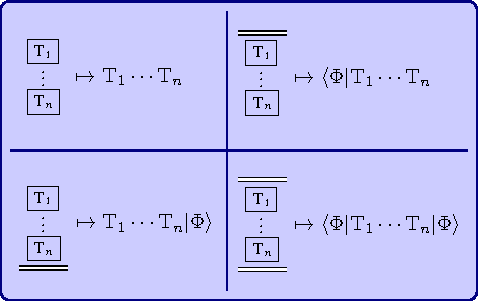
\includegraphics[height=5.7cm]{figs/diagram-ordering.pdf}
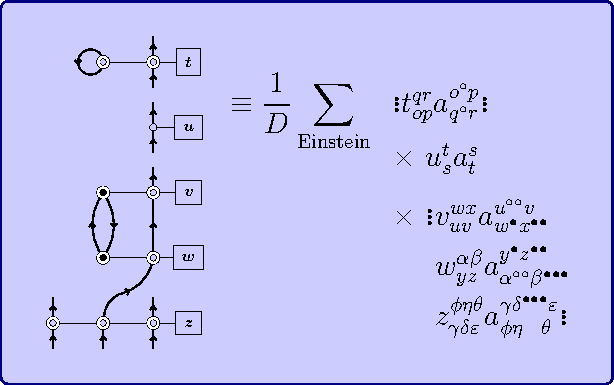
\includegraphics[height=5.7cm]{figs/diagram-example.pdf}
\caption{(a) vertical ordering of a diagram, showing four possible cases of vacuum state bra/ket bookends.
(b)~a~generic example of a diagram, along with its corresponding algebraic term.}
\end{figure}

\begin{ex}
The degeneracy of the product in fig~\ref{fig:diagram-example}(b) is $D=2!2!3!$, so the diagram's degeneracy factor is $\sfr{1}{D}=\sfr{1}{24}$.
\end{ex}

\begin{ex}
Applying the rules of interpretation to a single un-contracted Goldstone operator: 1.~tells us that all lines are summed over, 3.~tells us that the expression has a factor of $\dfr{1}{(m!)^2}$ in front
\begin{align*}
&&
\diagram{
  \node[draw] (label) at (-0.7,0) {\bm{v}};
  \node[dot=white] (v1) at (0,0) {};
  \node[dot=white] (v2) at (1,0) {};
  \node (dots) at (1.75,0) {$\cdots$};
  \node[dot=white] (vn) at (2.5,0) {};
  \draw (label)--(v1)--(v2)--(dots)--(vn);
  \draw[->-] (v1) to ++(0,+0.5);
  \draw[->-] (v2) to ++(0,+0.5);
  \draw[->-] (vn) to ++(0,+0.5);
  \draw[-<-] (v1) to ++(0,-0.5) coordinate[below left=0.1cm and 0.1cm] (startbrace);
  \draw[-<-] (v2) to ++(0,-0.5);
  \draw[-<-] (vn) to ++(0,-0.5) coordinate[below right=0.1cm and 0.1cm] (endbrace);
}
\equiv
  \pr{\tfr{1}{m!}}^2
  \sum_{\substack{p_1\cd p_m\\q_1\cd q_m}}
\diagram{
  \node[draw] (label) at (-0.7,0) {\bm{v}};
  \node[dot=white] (v1) at (0,0) {};
  \node[dot=white] (v2) at (1,0) {};
  \node (dots) at (1.75,0) {$\cdots$};
  \node[dot=white] (vn) at (2.5,0) {};
  \draw (label)--(v1)--(v2)--(dots)--(vn);
  \draw[->-] (v1) to ++(0,+0.45) node[above] {$p_1$};
  \draw[->-] (v2) to ++(0,+0.45) node[above] {$p_2$};
  \draw[->-] (vn) to ++(0,+0.45) node[above] {$p_m$};
  \draw[-<-] (v1) to ++(0,-0.45) node[below] {$q_1$};
  \draw[-<-] (v2) to ++(0,-0.45) node[below] {$q_2$};
  \draw[-<-] (vn) to ++(0,-0.45) node[below] {$q_m$};
}
\equiv&\
  \pr{\tfr{1}{m!}}^2
  \sum_{\text{Einstein}}
  \ol{v}_{p_1p_2\cdots p_m}^{q_1q_2\cdots q_m}
  a^{p_1p_2\cdots p_m}_{q_1q_2\cdots q_m}
\end{align*}
which shows that the diagram is exactly equal to $V$, including the correct summations and the correct scalar factor.
\end{ex}

\begin{ex}
Similarly, for a diagram consisting of a single Hugenholtz operator, we get
\begin{align*}
&&
\diagram{
  \node[draw,circle] (label) at (0,0) {\bm{v}};
  \draw[->-] (label.140) -- ++(140:0.5);
  \draw[->-] (label.120) -- ++(120:0.5);
  \draw[->-] (label.40)  -- ++(40:0.5);
  \node at (70:0.55) {$\cdot$};
  \node at (80:0.55) {$\cdot$};
  \node at (90:0.55) {$\cdot$};
  \draw[-<-] (label.220) -- ++(220:0.5);
  \draw[-<-] (label.240) -- ++(240:0.5);
  \node at (270:0.55) {$\cdot$};
  \node at (280:0.55) {$\cdot$};
  \node at (290:0.55) {$\cdot$};
  \draw[-<-] (label.320) -- ++(320:0.5);
}
\equiv
  \pr{\tfr{1}{m!}}^2
  \sum_{\substack{p_1\cd p_m\\q_1\cd q_m}}
\diagram{
  \node[draw,circle] (label) at (0,0) {\bm{v}};
  \draw[->-] (label.140) -- ++(140:0.5) ++(140:0.2) node {$p_1$};
  \draw[->-] (label.120) -- ++(120:0.5) ++(120:0.2) node {$p_2$};
  \node at (70:0.55) {$\cdot$};
  \node at (80:0.55) {$\cdot$};
  \node at (90:0.55) {$\cdot$};
  \draw[->-] (label.40)  -- ++(40:0.5)  ++(40:0.25)  node {$p_m$};
  \draw[-<-] (label.220) -- ++(220:0.5) ++(220:0.2) node {$q_1$};
  \draw[-<-] (label.240) -- ++(240:0.5) ++(240:0.2) node {$q_2$};
  \node at (270:0.55) {$\cdot$};
  \node at (280:0.55) {$\cdot$};
  \node at (290:0.55) {$\cdot$};
  \draw[-<-] (label.320) -- ++(320:0.5) ++(320:0.25) node {$q_m$};
}
\equiv
  \pr{\tfr{1}{m!}}^2
  \sum_{\text{Einstein}}
  \ol{v}_{p_1p_2\cdots p_m}^{q_1q_2\cdots q_m}
  a^{p_1p_2\cdots p_m}_{q_1q_2\cdots q_m}
\end{align*}
where we have assigned dummy indices of summation in left-to-right order.
\end{ex}

\begin{dfn}
\thmtitle{Equivalent operators}
Two copies of the an $m$-electron operator in a diagram are considered \textit{equivalent} if they are connected to exactly the same number 
\end{dfn}



\begin{dfn}
\thmtitle{Adjacent}
Two lines which are incident with the same vertex are called \textit{adjacent}.
\end{dfn}

\begin{dfn}
\thmtitle{Path}
A sequence of adjacent lines is called a \textit{path}.
Each path has either two external lines, in which case it is an \textit{open path}, or none, in which case it is a \textit{closed path}.
A closed path is also known as a \textit{loop}.
\end{dfn}

\begin{dfn}
\thmtitle{Contraction pattern}
\end{dfn}


\subsection{Antisymmetrized Goldstone diagrams}

\begin{rmk}
Because we always include a degeneracy factor $\prod_i\fr{1}{n_i!}$, any diagram corresponds to a sum \ul{over all unique terms}.
This means that, in expanding vac-normal operators in terms of $\F$-normal ones, the expansion will always be balanced if we include only the symmetry-unique diagrams.
\end{rmk}

\begin{drv}
\thmtitle{Counting the degeneracy of a contraction pattern}
For the sake of counting the degeneracy of a contraction pattern, we can decompose the figure into subsets $\{S_1,\cd,S_m\}$ of lines which are equivalent in the diagram components -- lines which have the same orientation and are connected to the same tensor.
For each $S_i$, let $\{S_i(0),S_i(1),\cd,S_i(m)\}$ be a partition into external lines $S_i(0)$ and contraction lines $S_i(j)$, where the lines from $S_i(j)$ are contracted with the lines from $S_j(i)$ in the final diagram.
Obviously, $|S_i(j)|$ must equal $|S_j(i)|$ and unless $S_i$ and $S_j$ have compatible orientations both sets must be empty, $S_i(j)=S_j(i)=\O$.
The degeneracy of the contraction pattern is given by the number of ways of partitioning each set of equivalent lines into external lines and contraction lines times the number of ways of forming each contraction between $S_i(j)$-$S_j(i)$ pairing, which is simply $|S_i(j)|!$.
This gives
\begin{align*}
  n_{\mr{ctr}}
=&\
  \prod_{i=1}^m
  {|S_i| \choose |S_i(0)|, |S_i(1)|,\cd, |S_i(m)|}
  \times
  \prod_{i=1}^m
  \prod_{j=i+1}^m
  |S_i(j)|!
=
  \prod_{i=1}^m
  \fr{|S_i|!}{|S_i(0)|!}
  \pr{
    \prod_{j=1}^{i-1}
    \fr{1}{|S_i(j)|!}
  }
\end{align*}
where the product $\prod_{i=1}^m\prod_{j=i+1}^m$ runs over $i,j$ pairs with $i<j$ and  $\ds{{n\choose k_1,\cd,k_m}}=\dfr{n!}{k_1!\cd k_m!}$ are multinomial coefficients.
\end{drv}

\begin{thm}
\thmstatement{
Consider a connected diagram composed of antisymmetrized operators.
Then the total degeneracy of the contraction pattern is
\begin{align}
&&
  \textnormal{(diagram weight)}
=
  \pr{
    \prod_i
    \fr{1}{\textnormal{component $i$ degeneracy}}
  }
\times
  \textnormal{(contraction degeneracy)}
\end{align}
}
\thmproof{


Number of contractions $=$ number of ways of partitioning each $S_i$ into an external set and $m-1$ sets for contraction with $S_j$, $j\neq i$.
}
\end{thm}


\begin{lem}
To illustrate this theorem, we can explicitly consider 
\begin{align*}
&&
\diagram{
% operator a
  \node[draw] (alabel) at (-0.7,0) {\bm{a}};
  \node[dot] (a1) at (0.0,0) {};
  \node (adots1) at (0.75,0) {\cd};
  \node[dot] (a2) at (1.5,0) {};
  \node[dot] (a3) at (2.5,0) {};
  \node (adots2) at (3.24,0) {\cd};
  \node[dot] (a4) at (4.0,0) {};
  \draw (alabel)--(a1)--(adots1)--(a2)--(a3)--(adots2)--(a4);
% operator b
  \node[dot] (b4) at (2.5,1) {};
  \node (bdots2) at (3.25,1) {\cd};
  \node[dot] (b3) at (4.0,1) {};
  \node[dot] (b2) at (5.0,1) {};
  \node (bdots1) at (5.75,1) {\cd};
  \node[dot] (b1) at (6.5,1) {};
  \node[draw] (blabel) at (7.2,1) {\bm{b}};
  \draw (blabel)--(b1)--(bdots1)--(b2)--(b3)--(bdots2)--(b4);
% lines
  \draw[->-] (a1) to ++(0,+1);
  \draw[->-] (a2) to ++(0,+1);
  \draw[->-] (a3) to     (b4);
  \draw[->-] (a4) to     (b3);
  \draw[-<-] (b2) to ++(0,-1);
  \draw[-<-] (b1) to ++(0,-1);
}
\end{align*}
Let $A$ be the set of lines leaving \bm{a} and let $B$ be the set of lines leaving \bm{b}.
Then the deneracy of this contraction pattern is.
\begin{align*}
&&
  d_{\mr{ctr}}
=
  {|A| \choose |A\cap B|}
  \cdot
  {|B| \choose |A\cap B|}
  \cdot
  |A\cap B|!
=
  \fr{|A|!|B|!}{|A\bs B|!|A\cap B|!|B\bs A|!}
\end{align*}
The degeneracies of \bm{a}, \bm{b}, and the diagram as a whole are
\begin{align}
&&
  d_{\bm{a}}
=
  |A|!
&&
  d_{\bm{b}}
=
  |B|!
&&
  d_{\mr{diag}}
=
  |A\bs B|!|A\cap B|!|B\bs A|!
\end{align}
which shows that $\dfr{d_{\mr{diag}}}{d_{\bm{a}}d_{\bm{b}}}=d_{\mr{ctr}}$.
\end{lem}


\end{document}
